\documentclass[a4paper]{article}
\usepackage[utf8x]{inputenc}
\usepackage[english]{babel}
\usepackage{a4wide}
\usepackage[pdftex,hidelinks]{hyperref}
\usepackage{float}
\usepackage{graphicx}
\usepackage{fancyhdr}
\usepackage{booktabs}
\usepackage{lastpage}
\usepackage{array}
\usepackage{tikz}
\usepackage{multirow}
\usepackage[normalem]{ulem}


\usetikzlibrary{arrows,positioning,automata,decorations.markings,shadows,shapes,calc}

\pagestyle{fancy}
\fancyhf{}

\rfoot{Page \thepage~of~\pageref{LastPage}}
\newcommand{\centered}[1]{\begin{tabular}{l} #1 \end{tabular}}
\newcommand\myworries[1]{\textcolor{red}{#1}}
\newcommand\mydoubts[1]{\textcolor{blue}{#1}}
\begin{document}

\title{Spy Kid}
\author{%
    \begin{tabular}{lll}
        95145 & Eva Verboom & \multirow{2}{*}{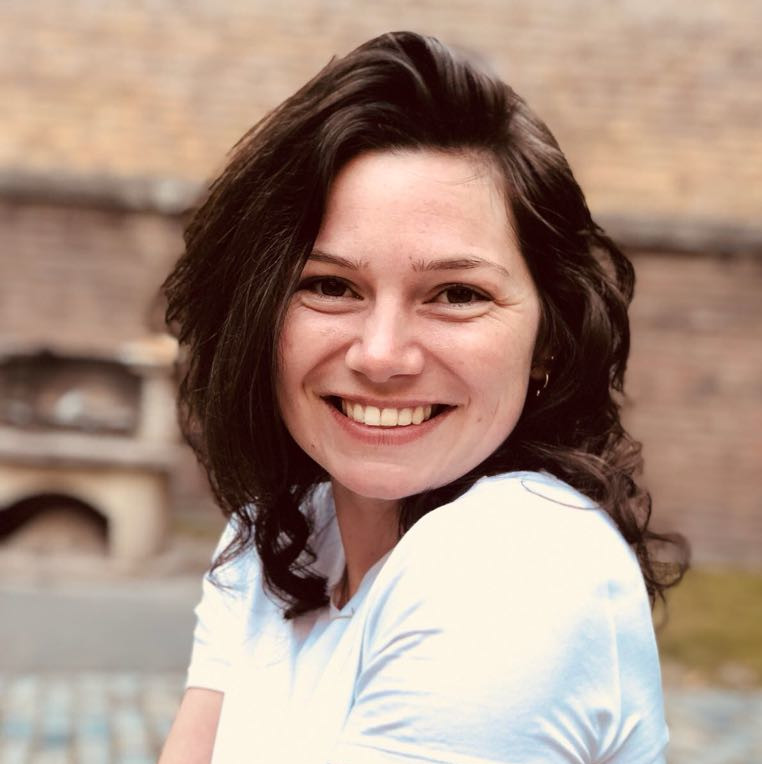
\includegraphics[height=3cm]{images/eva_square.jpeg}} \\
        \multicolumn{2}{l}{\text{eva.verboom@tecnico.ulisboa.pt}} & \\[2.1cm]
        95383 & Felipe Gorostiaga &
        \multirow{2}{
\includegraphics[height=3cm]{images/felipe.jpg}} \\
        \multicolumn{2}{l}{felipe.gorostiaga@tecnico.ulisboa.pt} & \\[2.1cm]
        97144 & Pedro Mendes &
        \multirow{2}{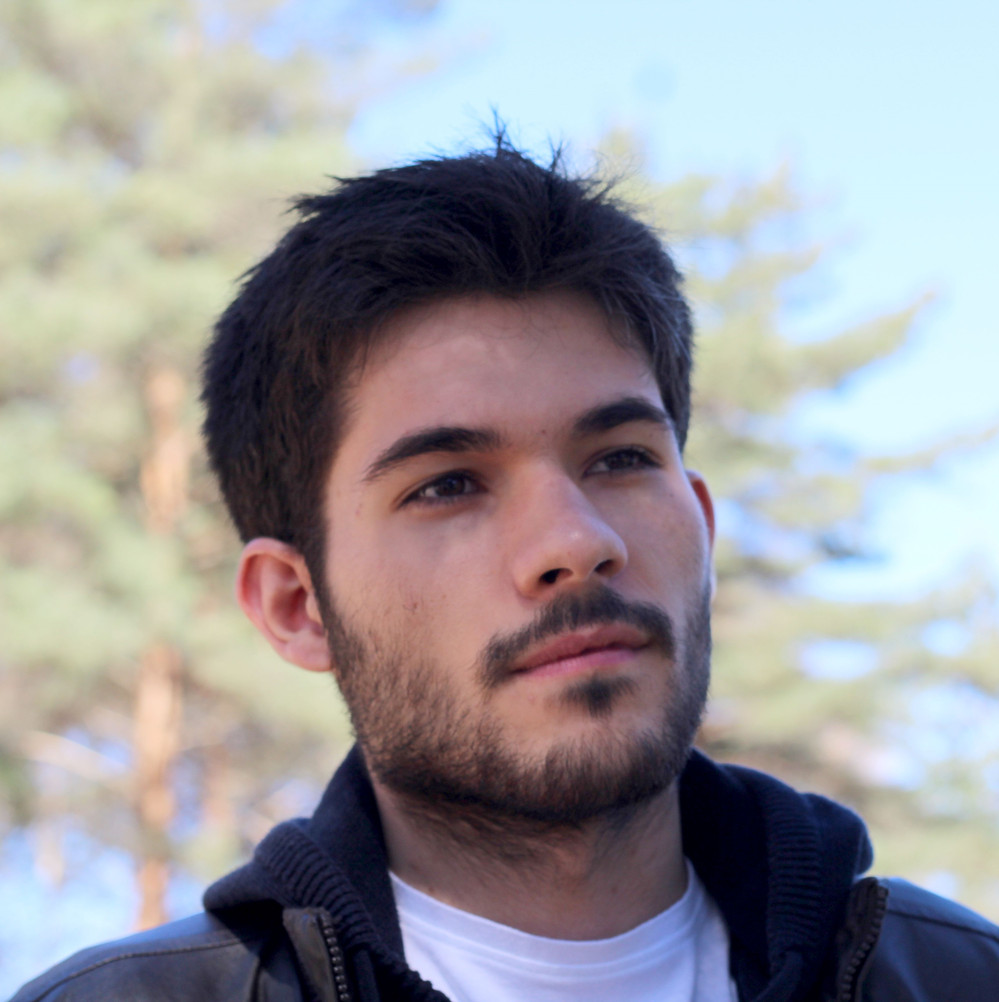
\includegraphics[height=3cm]{images/pedro.jpg}} \\
        \multicolumn{2}{l}{pedromendesfc@tecnico.ulisboa.pt} & \\[2.1cm]
    \end{tabular}
}

\date{\today}

\begin{titlepage}

    %título
    \begin{center}
        \begin{minipage}{0.75\linewidth}
            \centering
            \vspace{1.5cm}
            %títulos
            \href{https://fenix.tecnico.ulisboa.pt/disciplinas/SIRS7/2019-2020/1-semestre}
            {\scshape\LARGE Network and Computer Security} \par
            \vspace{1cm}
            {\scshape\Large Alameda} \par
            \vspace{1cm}
            {\scshape\Large Group 28} \par
            \vspace{1.5cm}

            \maketitle
        \end{minipage}
    \end{center}

\end{titlepage}

\tableofcontents
\thispagestyle{empty}
\newpage
\setcounter{page}{1}

\pagebreak

%% I  Problem (Given the chosen scenario, where is security necessary? What is the main problem being solved? Use around 200 words)
\section{The Problem}
During this project we have been working on the development of a secure child location application called \emph{SpyKid}. As a guardian, one might want to track your children to ensure that they are not straying too far from where they are supposed to be and in case something is wrong, to find them. Of course, the location of a person, especially a child, is very sensitive information. Nobody should to be able to track your children, to find them or misuse the information in any way. Therefore, accessing the information should only be possible for authorised guardians and secure communication of the child's location is required as well as secure storage on remote servers. This implies that also the servers that are storing the location data and people that have access to these servers should not be able to read the location of any child. Besides, proper authentication of all clients is required in order to give the right people access to the right information. In the following the explicit requirements of the application and the trust assumptions made in the development will be discussed. 

%% a. Requirements (Which security requirements were identified for the solution? Present as a list)
\subsection{Requirements}

The security requirements needed to solve this problem can be defined as follows:
\begin{itemize}
    \item The system must maintain the confidentially of all data that is classified as confidential;
    \item The system must identify users in a reliable way;
    \item The system must only show data to users if they are authorised to access that particular data;
    \item The system must not allow anyone to fake localisation data;
    \item The system must not allow anyone to replay old packets;
    \item The system must add timestamps to the location broadcasted by the child's device;
    \item The system must use secure communication channels to exchange data between the server and the clients;
    \item The system must prefer secrecy over performance.
\end{itemize}

%% b. Trust assumptions (Be explicit about trust relationships. Who will be fully trusted, partially trusted, or untrusted)
\subsection{Trust Assumptions}
There are three groups of actors to be distinguished here: the children, the guardians and the external servers. Both children and guardians are fully trusted by the system, after they have been authenticated by the system. The external servers are be partially trusted. This implies that we trust the server to store and send data in a correct manner and keep the system running, but we do not allow the server to read data associated with the location of a child. All other actors that can in some way have access to the data are not trusted by the system.

%% Proposed solution (overview with diagram and explanation with around 200 words or less)
\section{Implementation}
This section describes the the configuration of the application: how different machines are connected, which communication channels are used and how they are used. Special attention is given to the security of the channels and protocols used by the system. 

%% a) Deployment (describe distinct machines and how they will be interconnected)
\subsection{Deployment}
The system consists of three moving parts:
\begin{itemize}
    \item A centralised server;
    \item Multiple guardian clients;
    \item Multiple child clients.
\end{itemize}
A graphical representation of the machines and the way they are interconnected is shown in \autoref{fig:graph}. To achieve secure communication between the server and the child and guardian clients, both require appropriate methods for authentication. Details of these methods will be discussed later on. 

\begin{figure}[ht!]
    \centering
    \tikzstyle{struct}=[%
    fill=white,
    draw=black,
    rectangle,
    drop shadow,
    minimum height=1.5cm,
    minimum width=1cm
]

\begin{tikzpicture}[font=\ttfamily,auto]
    \node (Server) [struct]{\textbf{\Large{Server}}};
    \node[below left = of Server] (Child) [struct]{\textbf{\Large{Child}}};
    \node[below right = of Server] (Guardian) [struct]{\textbf{\Large{Guardian}}};

    \draw[->, very thick, to path={|- (\tikztotarget)}] (Child.north) to (Server.west)
        node[above left = 0.3cm and 0.1cm] {\texttt{location beacon}};

    \draw[->, very thick, to path={|- (\tikztotarget)}] (Guardian.north) to (Server.east)
        node[above right = 0.3cm and 0.1cm] {\texttt{child location requests}};

    \draw[->, very thick, to path={|- (\tikztotarget)}] (Server.south) to (Guardian)
        node[below right = 2cm and -2.1cm of Server] {\texttt{child locations}};

    \draw[<->, densely dotted, very thick, draw=blue]
        (Child.south east) to[bend right=30] (Guardian.south west)
        node[below left = 0.6cm and 0.5cm] {\texttt{shared secret}};

\end{tikzpicture}

    \caption{Diagram of the System}\label{fig:graph}
\end{figure}

The main technology used for developing the applications is Android Studio \cite{android_studio}, using Java's Security \cite{java_security} and Cryptography \cite{javax_crypto} packages and written mostly in Kotlin \cite{kotlin} and part in Java. For the server PostgreSQL \cite{postgres} is used as the database and Rust \cite{rust} as the programming language for being a memory safe and high performing language. All of which are tested and stable before starting this project.

%% Secure channel(s) to configure (identify communication entities; existing library/tool to use;
%% what keys will exist and how will they be distributed)
\subsection{Secure channels}
First of all, a guardian should establish authentication with the server. This is done with a username and a local only password, which is always hashed before sending it to the server. Besides, the username is encoded in a byte-array and appended to the password before hashing as a salt, in order to prevent rainbow-table attacks. Communication with the server is done over TCP with session keys, more on this in the next section.  

The child and guardian clients need to agree on a private key that only they know, to encrypt every piece of data they send to the server. In order for the agreement of the keys to not be intercepted, this agreement is made physically. This is implemented by generating a 256-bit key with random values with the \texttt{SecureRandom} class \cite{secure_random} from the \texttt{java.security} package and storing it in a file on the device. Sharing the key is done by translating the key into a QR code in the guardian client, this code can then be scanned by a child application and also stored in a file as their shared secret. Afterwards the child client establishes a secure channel with the server using the same method the guardian client uses.

%% Secure protocol(s) to develop (identify communication entities; language to use for
%% implementation; what keys will exist and how will they be distributed)
\subsection{Secure Protocols}
All symmetric encryption and decryption done in this application will use a 256-bit key and follow the AES encryption algorithm with Cipher Block Chaining mode as is recommended by the Android Developer Community \cite{cipher_recommendation}. We are using PKCS5 padding because OpenSSL \cite{openssl} uses this by default. Encryption and decryption is done using the \texttt{javax.crypto} package on the Android clients and OpenSSL on the server. 

Effectively the entities that interact in the system are only the child and guardian clients, the server will only serve safe remote storage for the data. By using a public private key pair for the server and username and password for the clients we ensure authenticity. The server's public key is vendored in the application to make sure it isn't intercepted. All data exchanged between clients and the server is encrypted using a session key. This key is generated by the client and then sent encrypted with the RSA algorithm combined in ECB mode without padding using the 2048-bit public key of the server. To ensure freshness the server responds with a challenge, in the form of a 32-bit random value. Every message sent by the client in this session will be post-fixed with the challenge and the server will ignore messages that don't match the challenge. From then on the communication is encrypted with this shared secret. The session key and challenge are to be used for one session only and will therefore be deleted on both ends after a session closes. 

By using symmetric key encryption for the location, the clients can ensure confidentiality of the location data sent from child to guardian, meaning the server can never read the location data sent to it. 

\section{Results}
%% Versions (Describe basic, intermediate and advanced versions of the work and when are they
%% expected to be achieved)
\subsection{Project Versions}
Before starting the project we determined what the Minimum Viable Product, the Intermediate and Advanced versions should consist of. In this section we will reflect on those lists of requirements and the strengths and weaknesses of the implementation. 

\subsubsection{Minimum Viable Product (MVP)}
We said the MVP of our product should consist of the following:
\begin{itemize}
    \item Guardian accounts which can be authenticated by the server;
    % Authentication is done with username and hashed password
    \item Guardians should be able to create accounts for their children;
    % Guardians share a secret with the child clients and children are registered at the server
    \item \sout{Child clients should be able to localise themselves outdoors;} (Moved to full feature release)
    \item A central server that communicates with all clients and authorises guardians to view the tracking data of their children;
    % Done
    \item Data should be sent and stored encrypted, such that only guardians are able to track the child and the server is unable to know the location.
    % Data is encrypted using AES/CBC/NoPadding with shared secret
\end{itemize}
We decided to move the localization of the child client to the advanced version of the project, since the goal of this project is to show how security practices are implemented and retrieving the location from an Android phone took more time than expected. The rest of the requirements were implemented as discussed in the previous section and are up to standard according to security recommendations. Though, the current implementation does have some weaknesses. It does not add MAC signatures to send messages and therefore does not fully guarantee integrity and there are no requirements posed on the passwords of users, such as length or usage of strange characters, which could lead to weak passwords and therefore increases vulnerability to brute-force attacks. Here lies room for improvement in a future version. 

\subsubsection{Intermediate version}
The intermediate version of our product was supposed to include:
\begin{itemize}
    \item \sout{Child clients should also be able to locate themselves indoors;} (Moved to full feature release)
    % Think this should work if location is working (later worry)
    \item \sout{Child clients should be able to send alerts when they press an SOS button or go out of safe zones;} (Moved to full feature release)
    % Method is there -> database implementation, interface (button)
    \item Guardians should know when a child broadcasted a certain location;
    % Timestamps send with locations
    \item Guardian clients should be able to receive alerts \sout{send by the child and} when the child did not broadcast for a certain period of time;
    % Check timestamps at the server
    \item \sout{Allow multiple guardians;} (Removed)
    % This should be easy to implement
    \item \emph{Provide history of the child's location}.
\end{itemize}
As mentioned before location related implementation is moved to the full feature release. Because the alerts are partly linked to the live location of the child, this requirement is also moved to the next version. Allowing multiple guardians turned out to bring a lot of implementation issues with it, such as requiring the synchronisation of multiple clients which would take up to much time and was therefore removed from the requirements. On the other hand, the feature providing the history of the child's location was moved from there to the intermediate version, since implementation turned out to be more straightforward. In order to be able to display the history and be able to send alerts related to broadcasting time of the child, every location update of a child client contains a timestamp. This timestamp is encrypted with the shared secret, together with the latitude and longitude of the child. When the guardian receives a location from the server, the application checks if the timestamp is within five minutes before the current time and if not then the guardian receives an alert. 

\subsubsection{Full Feature Release}
Finally, we wanted the full feature release to extend the product with:
\begin{itemize}
    \item \sout{Login as a user should be done using two-factor authentication;} (Removed)
    % Think we should leave this, unless Filipe thinks it's easy to implement
    \item \emph{Child clients should be able to localize themselves};
    \item Child clients should be able to send alerts when they press an SOS button \sout{or go out of safe zones}; (Partly removed)
    \item \sout{Provide history of the child's location.} (Moved to intermediate version)
    % Should be okay to implement
\end{itemize}
For the final release we managed to retrieve the location of the mobile device of a child client and send it in the same secure way as before. We also managed to create an SOS button in the child application, which causes an alert on the guardian side when pressed: when the child presses the button it sends a \emph{flagged} location. The application on the guardians phone checks every location for this flag and if it is true alerts the guardian that his child is in need. Unfortunately, we did not have time to implement the structures required to set a safe-zone. Next to that, due to time restrictions and our belief that for this particular application it does not affect the security and assuming parents will keep their phone close by, two-factor authentication is cut from the list of features.

%% Effort commitments (table containing one row per week until the submission date; and one
%% column per group member with expected activities for the given week; some cells may be left
%% blank because of work in other courses)
\subsection{Effort Commitments}
The table below describes the activities each member of the team committed to during the project. This division of tasks is general and all team members also committed to helping each other where needed. During the middle of the project, we ended up about a week behind schedule since the basic version took more time then we expected. Though, in the last two weeks of the project we managed to catch up and finish most of the features we intended the application to have.
\begin{center}
\begin{tabular}{c m{3.7cm} m{3.7cm} m{3.7cm}}
    \toprule
    Week & Eva & Felipe & Pedro\\ \toprule
    28/10---3/11 & Basic non secure child client & Basic non secure guardian client & Basic non secure server \\\midrule
    4/11---10/11 & Basic secure child client and testing & Basic secure guardian client and testing & Basic secure server and testing\\\midrule
    11/11---17/11 & Intermediate child client & Intermediate guardian client & Intermediate secure server\\\midrule
    18/11---24/11 & Test intermediate child client & Test intermediate guardian client & Test intermediate secure server\\\midrule
    25/11---1/12 & Advanced child client and general outlines report & Advanced guardian client & Advanced server\\\midrule
    2/12---8/12 & Testing final product & Testing final product & Testing final product\\\midrule
    9/12---15/12 & Finishing report & Finishing report & Finishing report\\\bottomrule
\end{tabular}
\end{center}

%% References (tools, libraries, etc. that will be used in the project. State if each tool has been
%% found/installed/tested at the time of proposal)
\bibliography{bibliography.bib}
\bibliographystyle{unsrt}

\end{document}